\fontfamily{\sfdefault}\selectfont
% XCircuit output "basic_pll.tex" for LaTeX input from basic_pll.ps
\def\putbox#1#2#3#4{\makebox[0.00000in][l]{\makebox[#1][l]{}\raisebox{\baselineskip}[0.00000in][0.00000in]{\raisebox{#2}[0.00000in][0.00000in]{\scalebox{#3}{#4}}}}}
\def\rightbox#1{\makebox[0.00000in][r]{#1}}
\def\centbox#1{\makebox[0.00000in]{#1}}
\def\topbox#1{\raisebox{-0.60\baselineskip}[0.00000in][0.00000in]{#1}}
\def\midbox#1{\raisebox{-0.20\baselineskip}[0.00000in][0.00000in]{#1}}
   \scalebox{1}{
   \normalsize
   \parbox{4.49167in}{
   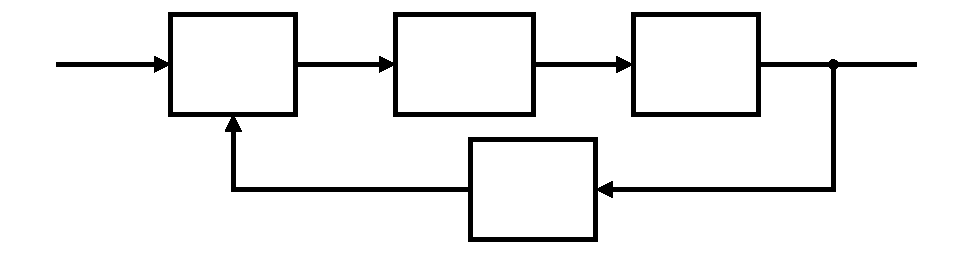
\includegraphics[scale=0.70000]{./figs/basic_pll.pdf}\\
   % translate x=320 y=488 scale 0.38
   \putbox{0.97300in}{0.82600in}{1.20}{PD}%
   \putbox{2.34500in}{0.24500in}{1.20}{$\div$ N}%
   \putbox{0.32900in}{0.97300in}{1.20}{$\Phi_{ref}$}%
   \putbox{3.71700in}{0.97300in}{1.20}{$\Phi_{out}$}%
   \putbox{1.90400in}{0.82600in}{1.20}{H$_{LF}$(s)}%
   \putbox{3.07300in}{0.82600in}{1.20}{VCO}%
   \putbox{1.49800in}{0.39200in}{1.20}{$\Phi_{div}$}%
   \putbox{1.52600in}{0.97300in}{1.20}{$\Phi_e$}%
   \putbox{2.54800in}{0.97300in}{1.20}{V$_{ctrl}$}%
   } % close 'parbox'
   } % close 'scalebox'
   \vspace{-\baselineskip} % this is not necessary, but looks better
\fontfamily{\rmdefault}\selectfont
